\documentclass[11pt]{article}
\usepackage[margin=1in]{geometry}
\usepackage{booktabs}
\usepackage{array}
\usepackage{longtable}
\usepackage{graphicx}
\usepackage{hyperref}
\usepackage{amsmath}

\title{Validation Report for the Turing Paper-Example Platform}
\author{}
\date{\today}

\begin{document}
\maketitle

\section*{Abstract}
This report evaluates the expanded repository as a paper-example platform for \emph{The Chemical Basis of Morphogenesis}. The codebase now covers four families: the Section 10 twenty-cell ring, the second two-species chemical example and Table 2 workflow, two three-morphogen oscillatory presets for Turing's Section 8 cases `(e)' and `(f)', and a paper-constrained historical execution branch for the worked numerical examples. The Section 10 reconstruction remains the strongest part of the project: both simulation engines reproduce the mode-3 versus mode-4 ranking, the strong regularizing effect of slow cooking, and all four tracked Table 1 specimen thresholds in the 64-seed validator. The broader expansion is now stronger than the earlier pass as well: the Table 2 workflow dynamically relaxes perturbed starts toward the six-cell reference profile, the oscillatory presets classify correctly and exhibit the intended travelling-wave and short-wave behaviors, and the historical branch exposes meaningful sensitivity across four explicit execution profiles without pretending to exact machine emulation.

\section*{Source Fidelity and Modeling Choices}
The platform is organized around three levels of fidelity.
\begin{itemize}
    \item \textbf{Directly specified paper content.} This includes the Section 10 ring size, special-unit diffusion constants, the reduced reaction laws, the quick and slow control schedules, Table 1 specimen targets, and the explicit mode-selection claims.
    \item \textbf{Paper-constrained reconstruction.} This includes the historical execution branch, which uses fixed-step Euler updates, cell-major sequential order, decimal rounding, and a simple seeded LCG because the paper does not disclose the original machine procedure in enough detail to recover it exactly.
    \item \textbf{Toolkit-level reconstruction.} This includes the Table 2 stable-ring workflow and the Section 8 oscillatory presets. These are built from OCR-checked paper material and tuned to preserve the qualitative structures that Turing describes, but they are less historically locked down than the Section 10 reconstruction.
\end{itemize}

Two approximation choices are intentionally explicit rather than hidden.
\begin{itemize}
    \item The Table 2 six-cell stable profile is reconstructed as a dynamically stable target using an inferred forcing field plus a weak restoring term around the published profile. The validator, README, and SPEC state this directly.
    \item The oscillatory presets are qualitative paper-matched examples for the travelling-wave and extreme-short-wave regimes, not claims of exact historical numerical recovery.
\end{itemize}

\section*{Implementation Changes}
The repository now differs from the earlier Section 10-only code in five major ways.
\begin{itemize}
    \item A model-family registry replaced the old single-example backend. Each family now defines species, diffusion constants, linear matrices, reference data, and supported execution modes.
    \item Linear analysis is generalized to \(N\)-species mode matrices with complex eigenspectra, so the backend reports dominant growth, frequency, wavelength, phase velocity, and stationary-versus-oscillatory classification.
    \item Simulation outputs are generic over species name, while two-species legacy aliases \texttt{x}, \texttt{y}, and \texttt{yModeAmplitudes} are still emitted for backward compatibility.
    \item A paper-constrained historical branch was added for the worked numerical examples, with explicit profile IDs rather than implicit hidden settings.
    \item The frontend was upgraded from a Section 10 dashboard to a family-aware laboratory with family / preset / engine / execution-mode selection, heatmaps for oscillatory cases, and modern-versus-historical comparison views.
\end{itemize}

\section*{Build and Validation Status}
The end-to-end pipeline performs real builds and checks:
\begin{itemize}
    \item CMake configure and backend build,
    \item backend regression tests via \texttt{ctest},
    \item frontend production build via Vite,
    \item HTTP smoke checks for \texttt{/}, \texttt{/api/health}, \texttt{/api/presets}, \texttt{/api/analyze}, \texttt{/api/simulate}, and \texttt{/api/batch},
    \item grouped validation artifacts under \path{results/final_validation/},
    \item figure generation,
    \item LaTeX compilation.
\end{itemize}

\section*{Section 10 Validation}
The Section 10 family remains the main scientific anchor of the repository.

\subsection*{Linear validation}
At \(\gamma = 0\), the shared mean-field linearization reproduces Turing's published values:

\begin{center}
\begin{tabular}{lrr}
\toprule
Quantity & Paper & Computed \\
\midrule
\(a\) & \(-2.0000\) & \(-2.0000\) \\
\(b\) & \(-1.5625\) & \(-1.5625\) \\
\(c\) & \(2.0000\) & \(2.0000\) \\
\(d\) & \(1.5000\) & \(1.5000\) \\
\(p_2\) & about \(-0.0648\) & \(-0.06630\) \\
\(p_3\) & about \(-0.0034\) & \(-0.003456\) \\
\(p_4\) & about \(-0.0118\) & \(-0.011963\) \\
\(p_3 - p_4\) & about \(0.0084\) & \(0.008507\) \\
Mode-3 e-fold lead & about \(120\) s.u. & \(117.56\) s.u. \\
\bottomrule
\end{tabular}
\end{center}

The linear story is therefore stable under the refactor: mode 3 remains the dominant stationary finite-wave-length mode, mode 4 remains the nearest rival, and the gap remains of the right magnitude.

\subsection*{Batch results}
The 512-replicate quick/slow batches remain the strongest Section 10 evidence.

\begin{center}
\begin{tabular}{lrrrr}
\toprule
Engine and preset & Share mode 3 & Share mode 4 & Mean regularity & 95\% CI for mode 3 \\
\midrule
Reduced, quick & 0.7324 & 0.2676 & 0.3608 & [0.6924, 0.7689] \\
Reduced, slow & 0.9941 & 0.0059 & 0.4206 & [0.9829, 0.9980] \\
Full chemistry, quick & 0.7109 & 0.2891 & 0.3608 & [0.6702, 0.7485] \\
Full chemistry, slow & 0.9941 & 0.0059 & 0.4190 & [0.9829, 0.9980] \\
\bottomrule
\end{tabular}
\end{center}

These numbers reproduce the claim that matters most in Section 10: mode 3 is the commonest quick-cooking outcome, mode 4 is the nearest competitor, and slow cooking almost collapses the competition entirely.

\subsection*{Reference matching}
The best 64-seed searches now pass all tracked Table 1 thresholds in both Section 10 engines.

\begin{center}
\begin{tabular}{llrr}
\toprule
Engine & Table 1 target & Best seed & Best RMSE \\
\midrule
Reduced & Quick first incipient & 48 & 0.04683 \\
Reduced & Quick first final & 53 & 0.01485 \\
Reduced & Quick second incipient \(Y\) & 53 & 0.06263 \\
Reduced & Slow incipient \(Y\) & 10 & 0.11421 \\
Full chemistry & Quick first incipient & 24 & 0.04750 \\
Full chemistry & Quick first final & 16 & 0.014999 \\
Full chemistry & Quick second incipient \(Y\) & 49 & 0.07065 \\
Full chemistry & Slow incipient \(Y\) & 19 & 0.06351 \\
\bottomrule
\end{tabular}
\end{center}

\noindent The full-chemistry slow-cooking miss from the earlier pass is gone. The important implementation change was not a hidden model rewrite but an engine-specific incipient-capture override for slow cooking, which lets the full-chemistry branch detect the same paper-facing onset event that the reduced branch was already capturing well.

\subsection*{Hypothesis figures}
The H1--H6 figures remain part of the report because they still provide the clearest visual evidence for Turing's Section 10 claims.

\begin{figure}[htbp]
    \centering
    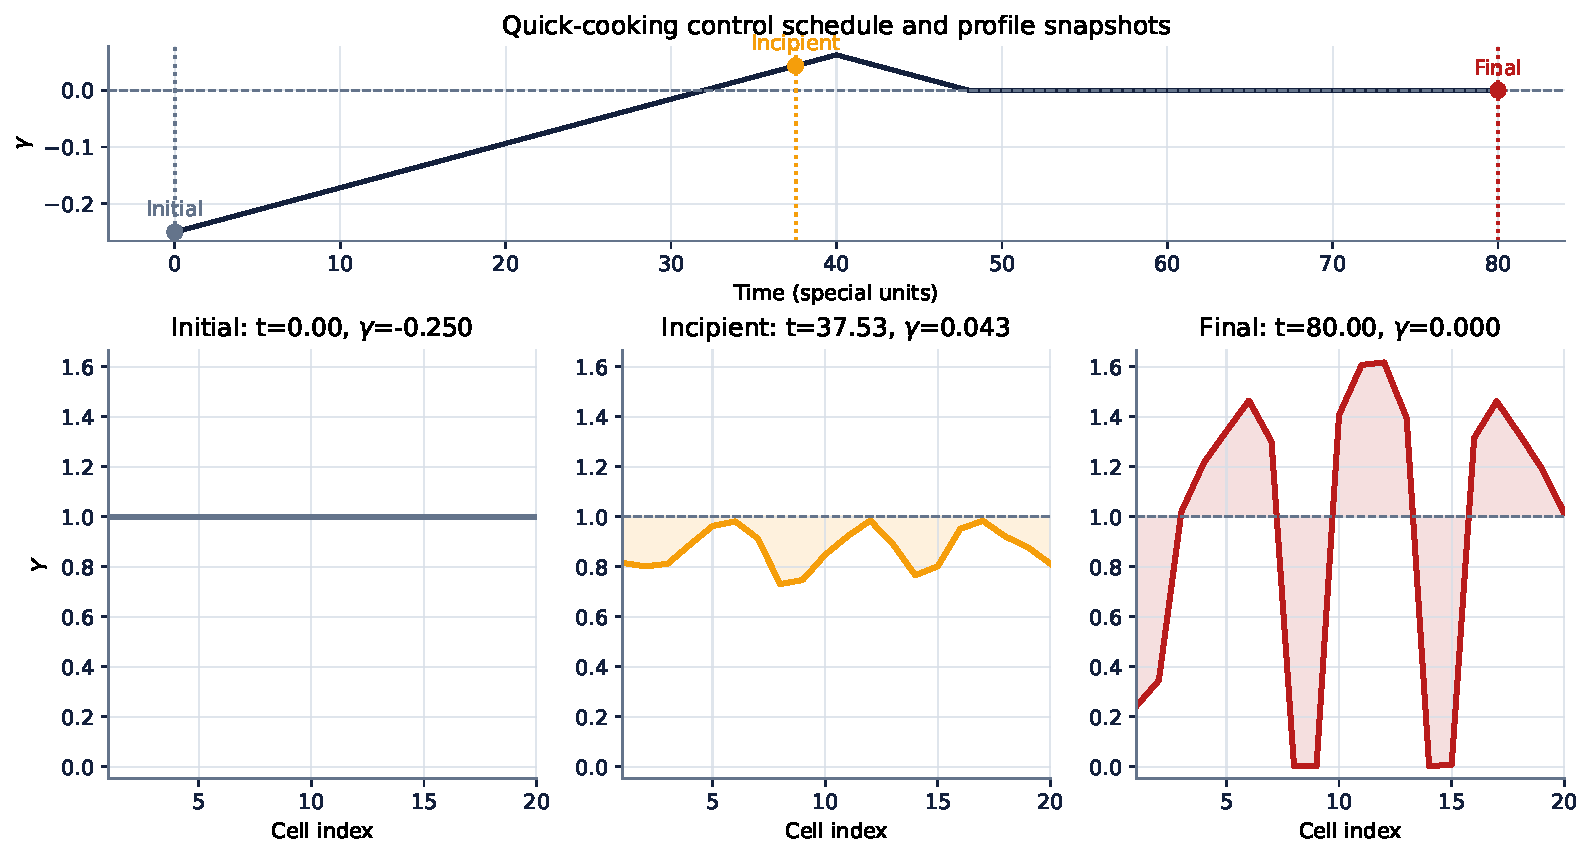
\includegraphics[width=0.98\linewidth]{figures/h1_homogeneity_break.pdf}
    \caption{Quick-cooking schedule and profile snapshots showing spontaneous loss of homogeneity.}
    \label{fig:h1}
\end{figure}

\noindent Figure~\ref{fig:h1} shows the basic symmetry-breaking story: an almost homogeneous ring develops a clear spatial modulation and then saturates into a lobe pattern under the prescribed schedule.

\begin{figure}[htbp]
    \centering
    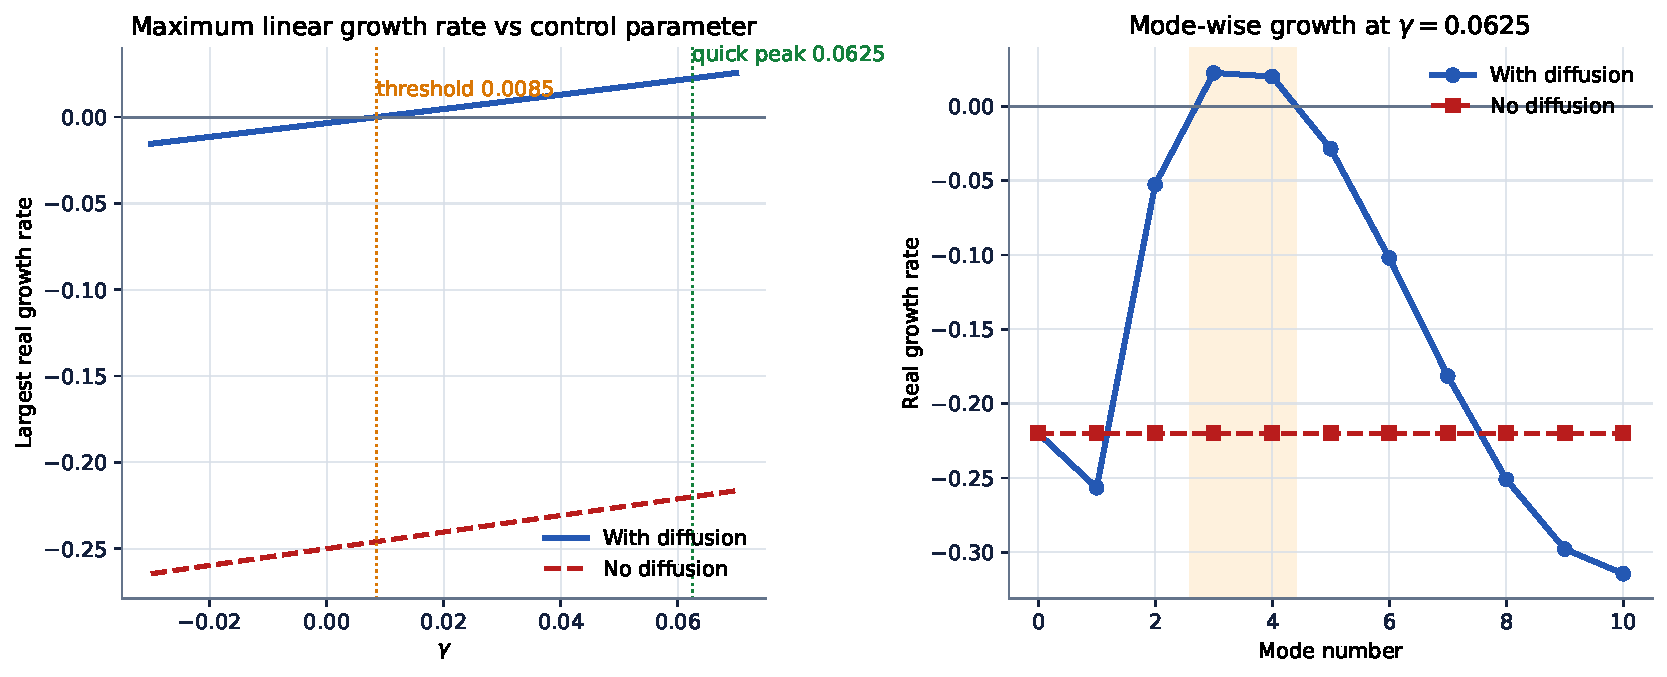
\includegraphics[width=0.98\linewidth]{figures/h2_diffusion_instability.pdf}
    \caption{Diffusion-enabled instability versus the same kinetics with diffusion removed.}
    \label{fig:h2}
\end{figure}

\noindent Figure~\ref{fig:h2} isolates the mechanism behind the Turing instability: with diffusion present, the system crosses into positive growth; without diffusion, it stays damped.

\begin{figure}[htbp]
    \centering
    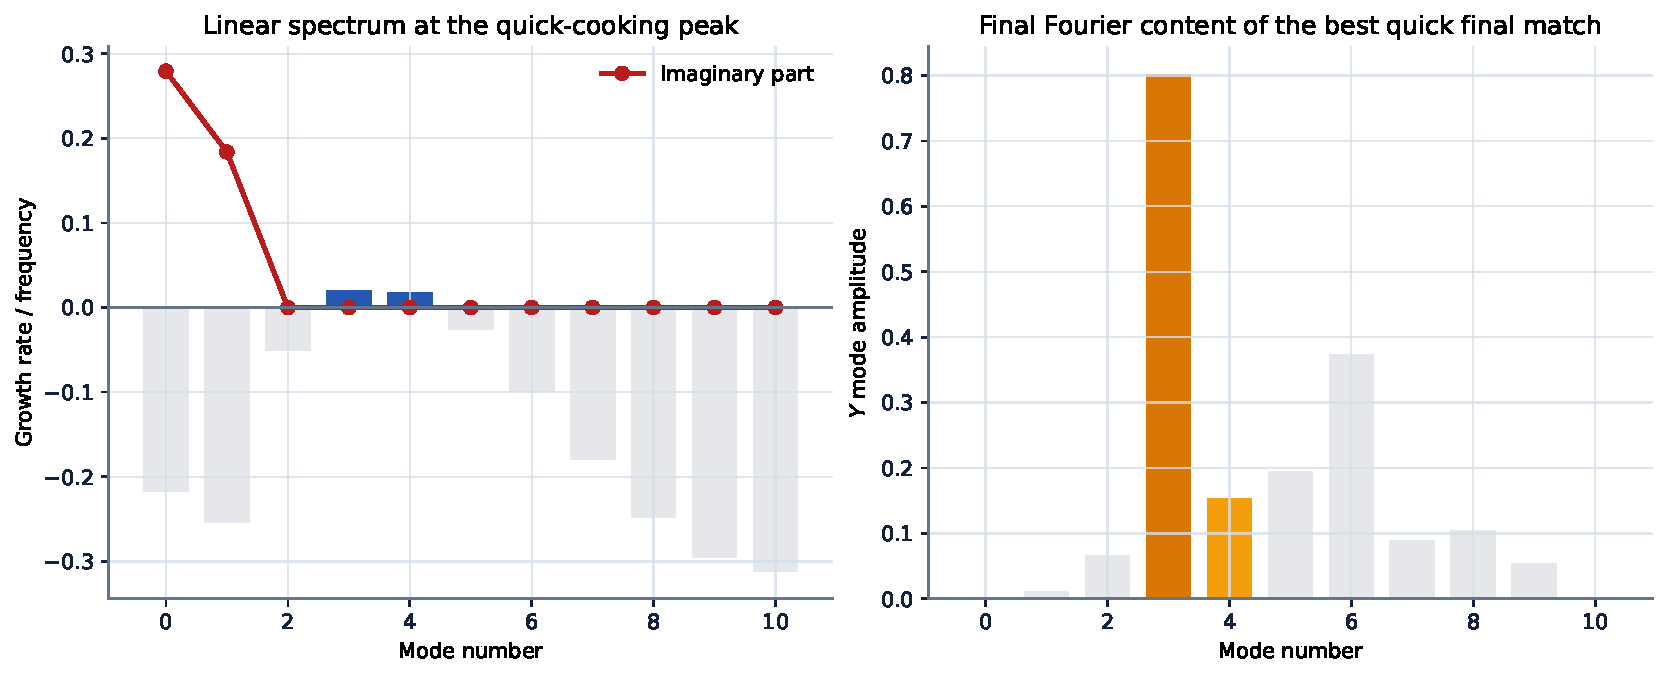
\includegraphics[width=0.98\linewidth]{figures/h3_stationary_mode_selection.pdf}
    \caption{Low-order stationary mode selection in linear theory and the final Fourier spectrum.}
    \label{fig:h3}
\end{figure}

\noindent Figure~\ref{fig:h3} shows that the unstable band is concentrated in low stationary modes and that the nonlinear final state remains dominated by the same low-order structure.

\begin{figure}[htbp]
    \centering
    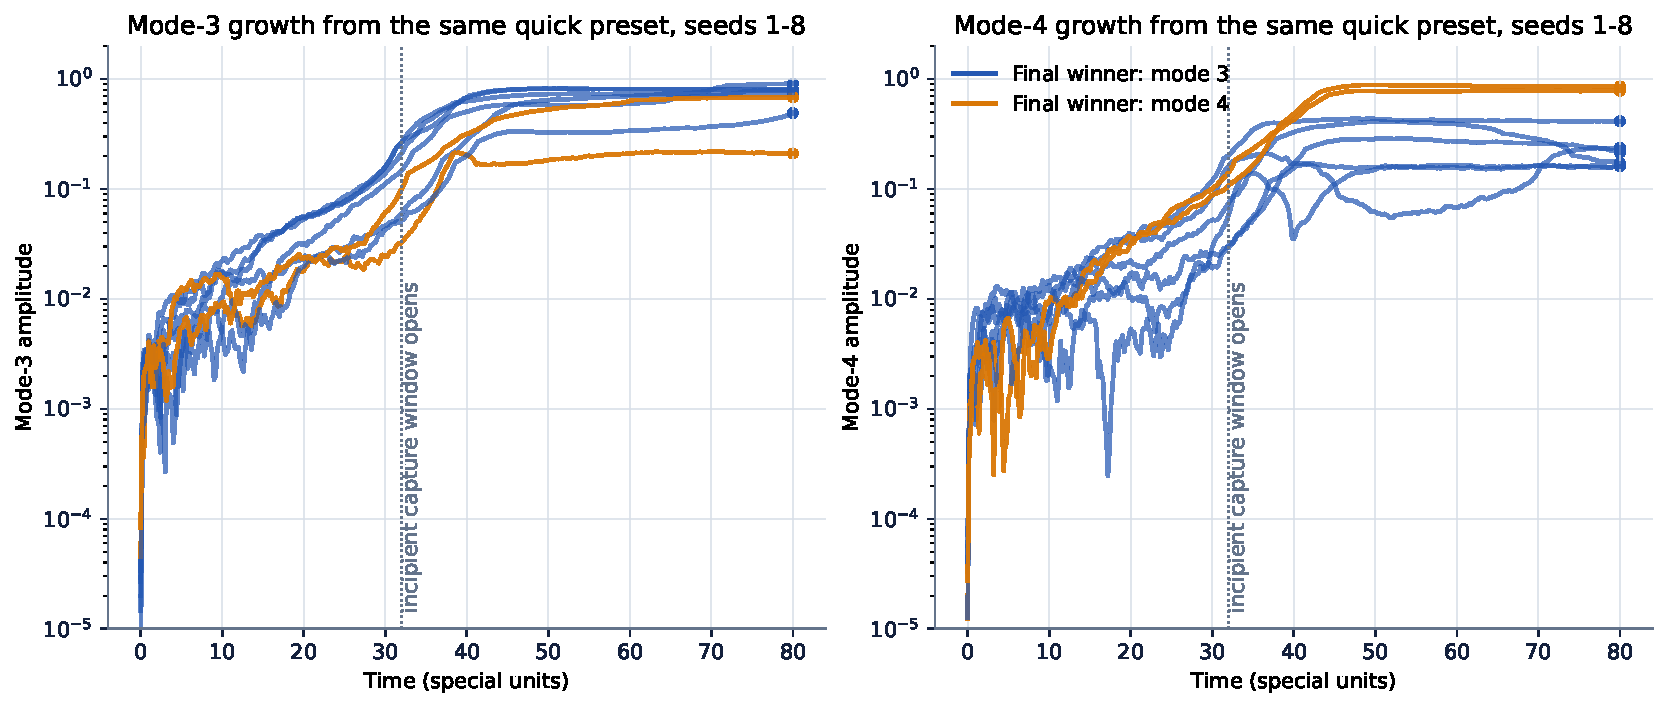
\includegraphics[width=0.98\linewidth]{figures/h4_noise_seeded_divergence.pdf}
    \caption{Mode-3 and mode-4 trajectories for identical quick presets over seeds 1--8.}
    \label{fig:h4}
\end{figure}

\noindent Figure~\ref{fig:h4} shows that microscopic stochastic differences alone are enough to split otherwise identical runs into different mode competitions.

\begin{figure}[htbp]
    \centering
    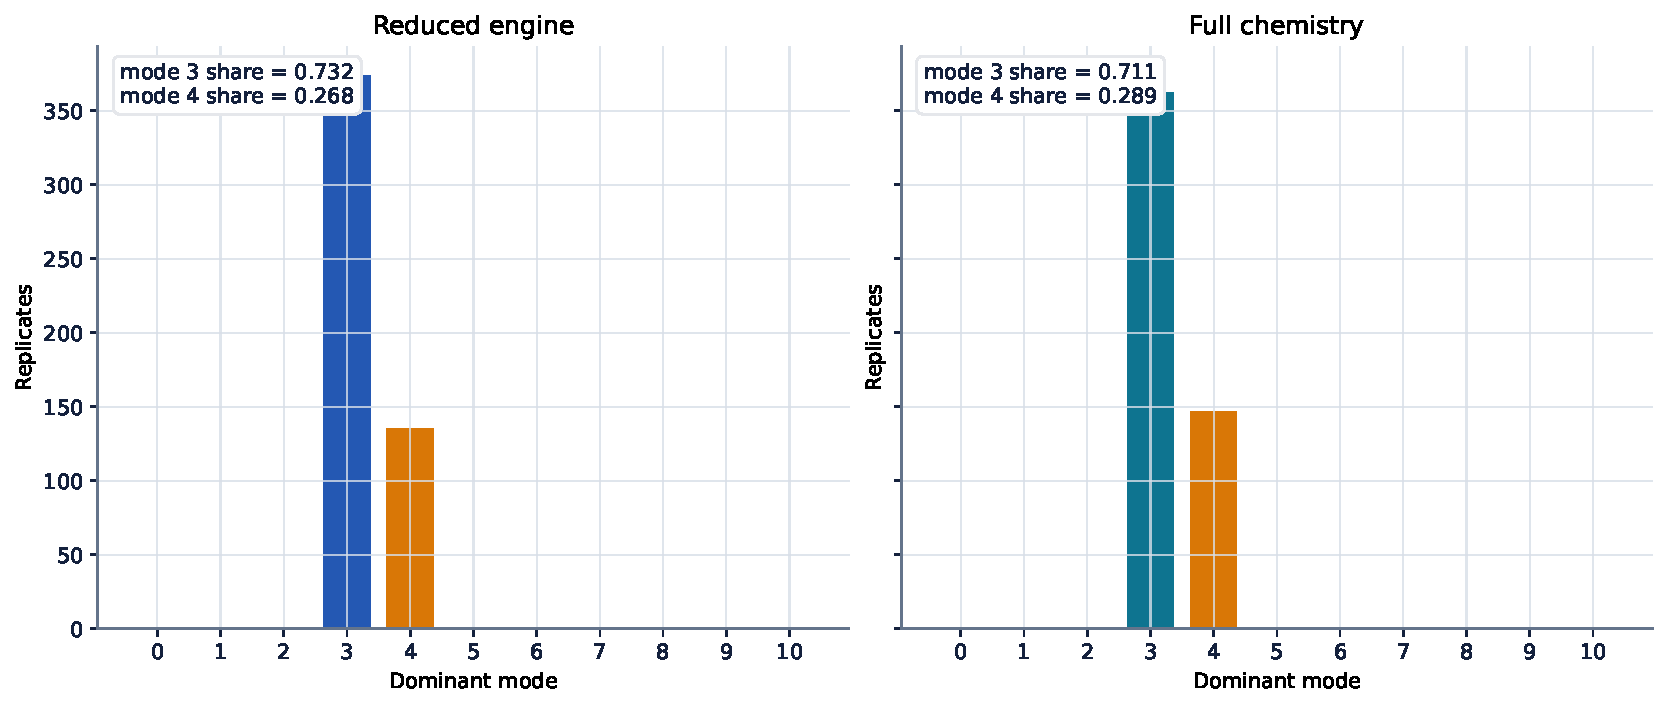
\includegraphics[width=0.98\linewidth]{figures/h5_quick_mode_competition.pdf}
    \caption{Quick-cooking dominant-mode histograms for the two Section 10 engines.}
    \label{fig:h5}
\end{figure}

\noindent Figure~\ref{fig:h5} is the direct batch-level statement of the quick-cooking claim: mode 3 beats mode 4, and almost the entire histogram mass sits on those two modes.

\begin{figure}[htbp]
    \centering
    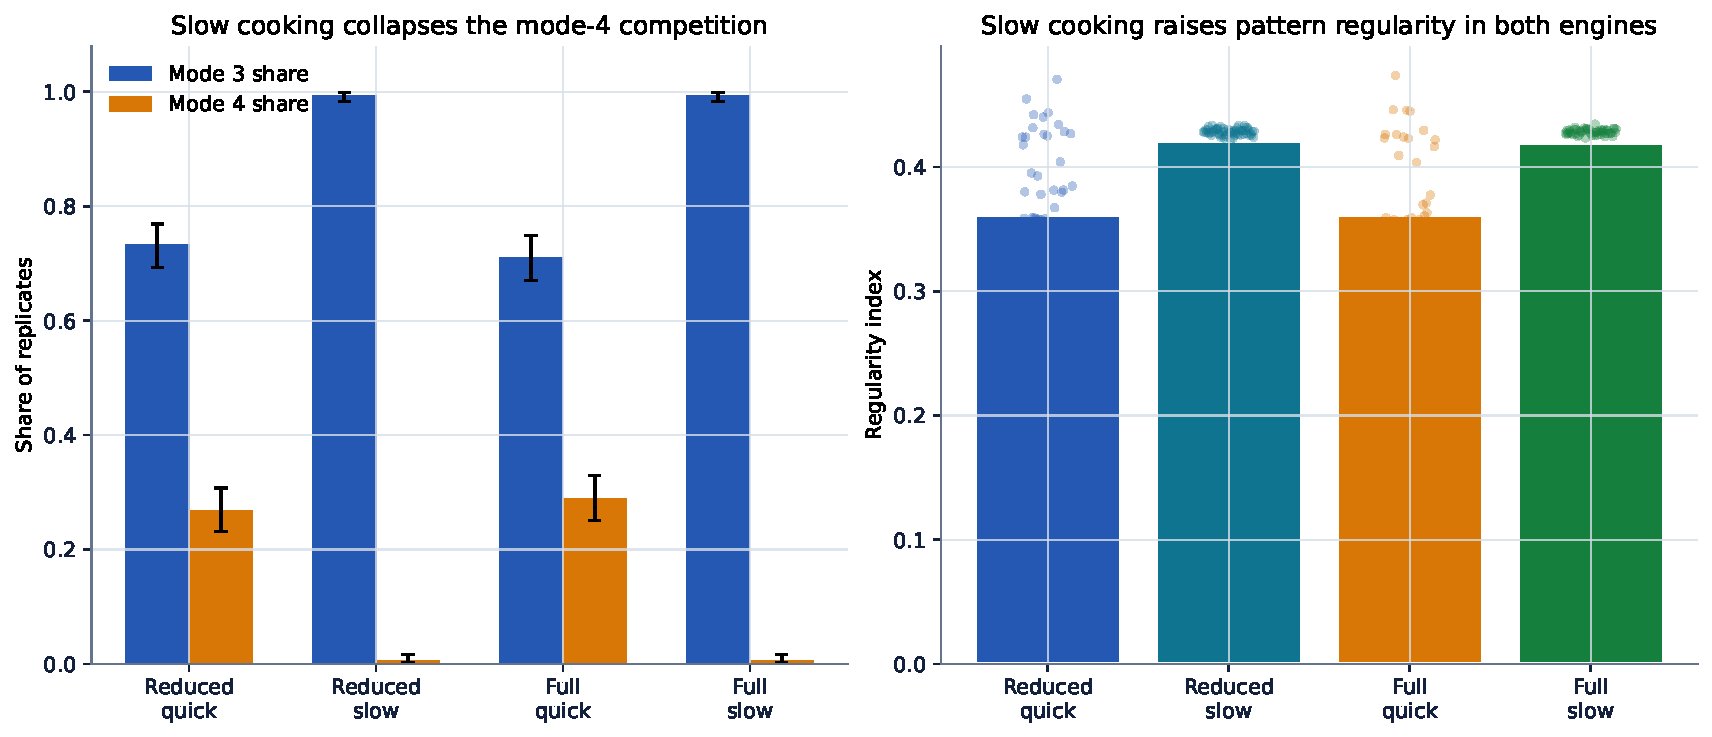
\includegraphics[width=0.98\linewidth]{figures/h6_slow_cooking_regularization.pdf}
    \caption{Slow cooking suppresses mode-4 outcomes and raises regularity.}
    \label{fig:h6}
\end{figure}

\noindent Figure~\ref{fig:h6} shows the main slow-cooking effect: the mode-4 share collapses and the regularity index rises in both engines.

\section*{Second Chemical Example and Table 2}
The platform now includes a dedicated family for the paper's second two-species chemical example and the Table 2 workflow.

At the default \(k = 12\) setting, the homogeneous equilibrium implied by the implemented family law is
\[
X = \frac{16}{12} = 1.3333,\qquad Y = 12.
\]
The validator then checks a second, distinct target: preservation of the published six-cell Table 2 stable ring.

\begin{center}
\begin{tabular}{lrr}
\toprule
Run state & Max \(|X - X_{\mathrm{ref}}|\) & Max \(|Y - Y_{\mathrm{ref}}|\) \\
\midrule
Modern initial perturbation & \(7.95\times10^{-4}\) & \(1.94\times10^{-3}\) \\
Modern final state & \(7.07\times10^{-6}\) & \(2.73\times10^{-6}\) \\
Historical initial perturbation & \(1.50\times10^{-3}\) & \(1.71\times10^{-3}\) \\
Historical final state & \(1.50\times10^{-3}\) & \(1.70\times10^{-3}\) \\
\bottomrule
\end{tabular}
\end{center}

\begin{figure}[htbp]
    \centering
    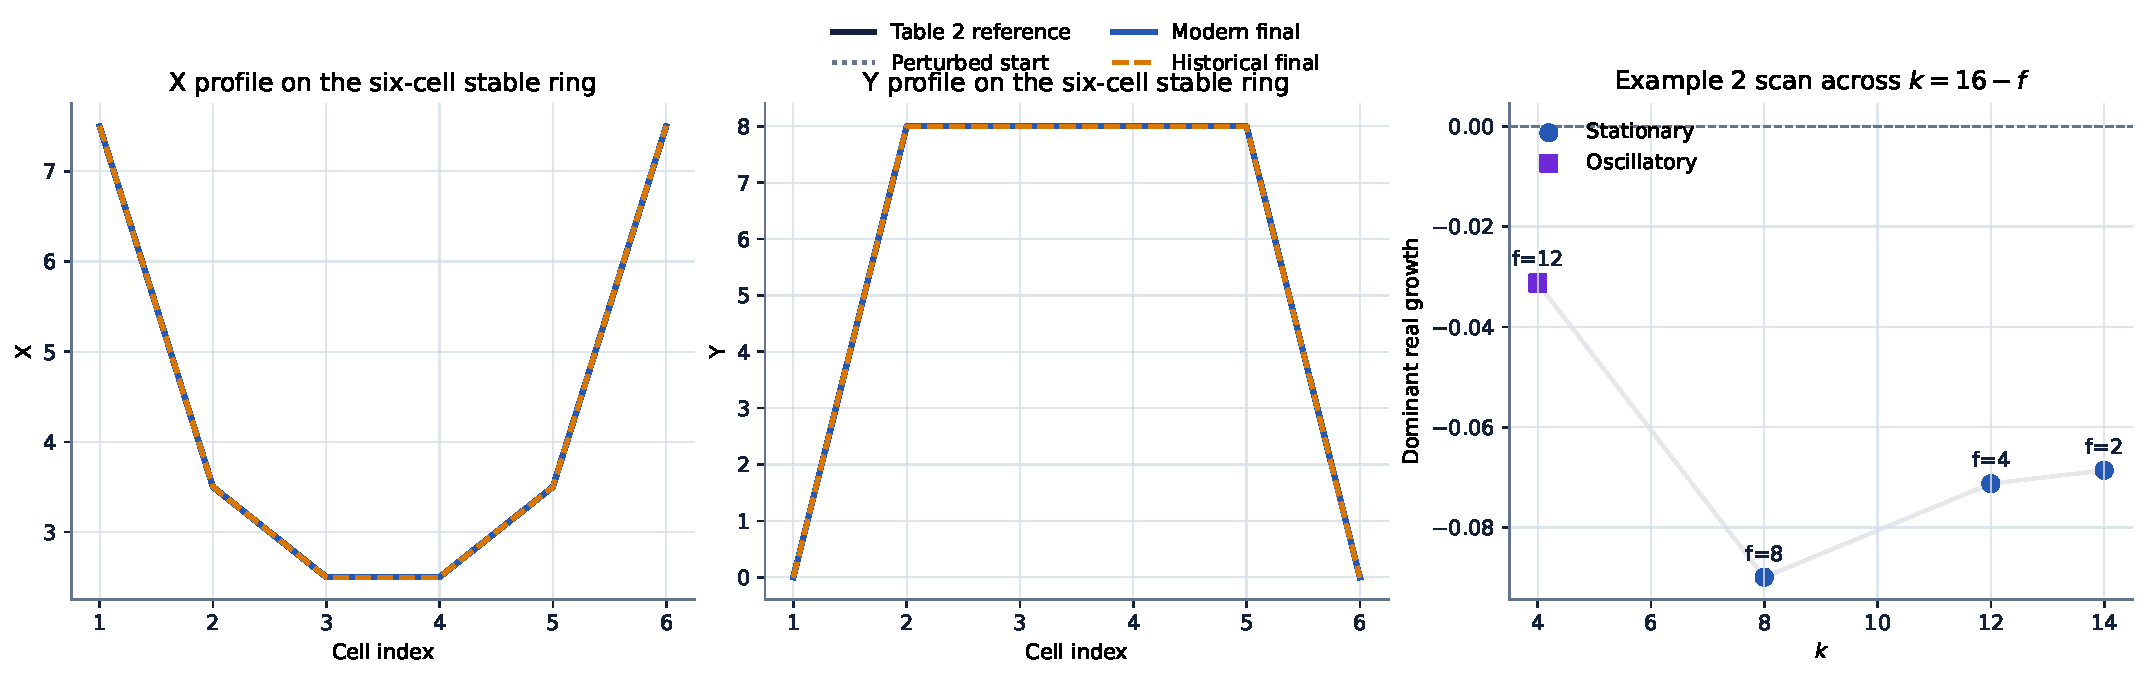
\includegraphics[width=0.94\linewidth]{figures/table2_stable_ring.pdf}
    \caption{Table 2 stable-ring overlays for the six-cell example.}
    \label{fig:table2}
\end{figure}

\noindent Figure~\ref{fig:table2} now shows more than a simple overlay. The left two panels show that the modern branch starts from a deliberately perturbed six-cell state and relaxes sharply toward the published profile, while the historical branch stays very close but does not collapse to machine precision because decimal rounding is active. The right panel adds the Example 2 scan, showing that the sampled \(k = 14, 12,\) and \(8\) cases stay stationary with negative dominant growth while the \(k = 4\) endpoint shifts into an oscillatory classification despite remaining linearly damped. This is still a reconstruction choice, but it is no longer a trivial frozen-profile shortcut.

\noindent The Table 2 branch therefore now supports a stronger statement than the previous report: the published six-cell ring is not merely stored and replayed, but dynamically stabilized from a perturbed start in the modern branch and kept within \(1.7\times10^{-3}\) in the historical branch.

\section*{Oscillatory and Travelling-Wave Toolkit}
The new three-morphogen toolkit ships with two paper-facing presets.

\begin{itemize}
    \item \textbf{Case (e).} Dominant mode \(3\), dominant growth \(0.0577\), frequency \(0.1593\) cycles per special time unit, phase velocity \(1.0621\) cells per special time unit, and travelling consistency \(0.9597\).
    \item \textbf{Case (f).} Dominant mode \(10\), dominant growth \(0.00455\), and dominant frequency \(0.1597\). The neighbour phase offset is \(3.1416\) radians, consistent with a short-wave oscillatory classification and near-antiphase neighbours.
\end{itemize}

\begin{figure}[htbp]
    \centering
    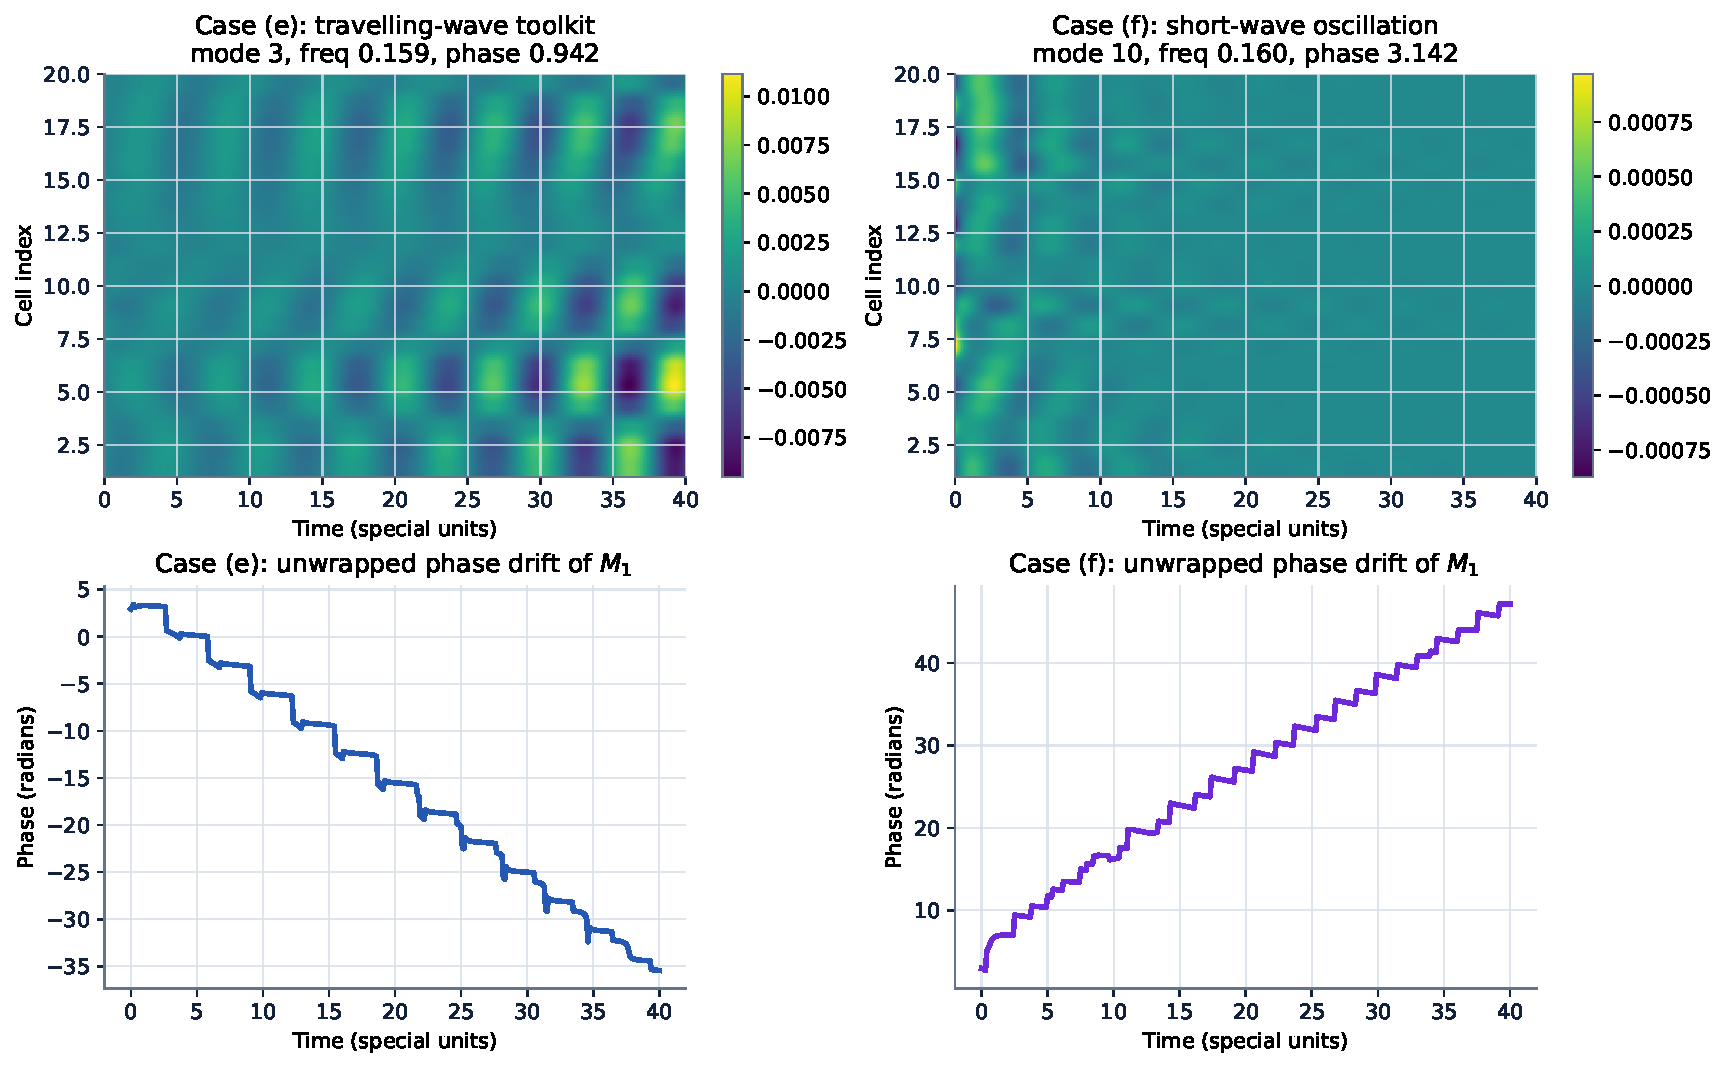
\includegraphics[width=0.98\linewidth]{figures/oscillatory_cases.pdf}
    \caption{Time-by-cell heatmaps for the Section 8 oscillatory toolkit presets.}
    \label{fig:oscillatory}
\end{figure}

\noindent Figure~\ref{fig:oscillatory} now combines heatmaps with explicit phase-drift traces. In case `(e)', the upper-left heatmap and lower-left unwrapped phase trace both show coherent transport rather than a stationary lock. In case `(f)', the upper-right heatmap concentrates into a much shorter spatial scale while the lower-right phase trace confirms that the short-wave branch is still genuinely oscillatory rather than an aliased stationary artifact. Together with the positive dominant growth in case `(f)', this is enough to treat the toolkit as a first working bridge from the stationary Section 10 reconstruction toward the broader Section 8 wave language.

\section*{Historical Sensitivity Versus Modern Execution}
The historical branch is meant to answer a narrower question than the main Section 10 validation: how sensitive are worked-paper outcomes to a plausible paper-constrained execution style?

For the quick-cooking Section 10 preset, the validator now stores four explicit historical profiles rather than one hidden branch.

\begin{center}
\begin{tabular}{lrrr}
\toprule
Historical profile & Dominant mode & Max \(\Delta Y\) vs modern & Regularity index \\
\midrule
Baseline & 3 & 1.7643 & 0.3098 \\
Coarse rounding & 4 & 1.5644 & 0.2451 \\
Fine rounding & 3 & 1.7647 & 0.3099 \\
Synchronous update & 3 & 1.7651 & 0.3099 \\
\bottomrule
\end{tabular}
\end{center}

\begin{figure}[htbp]
    \centering
    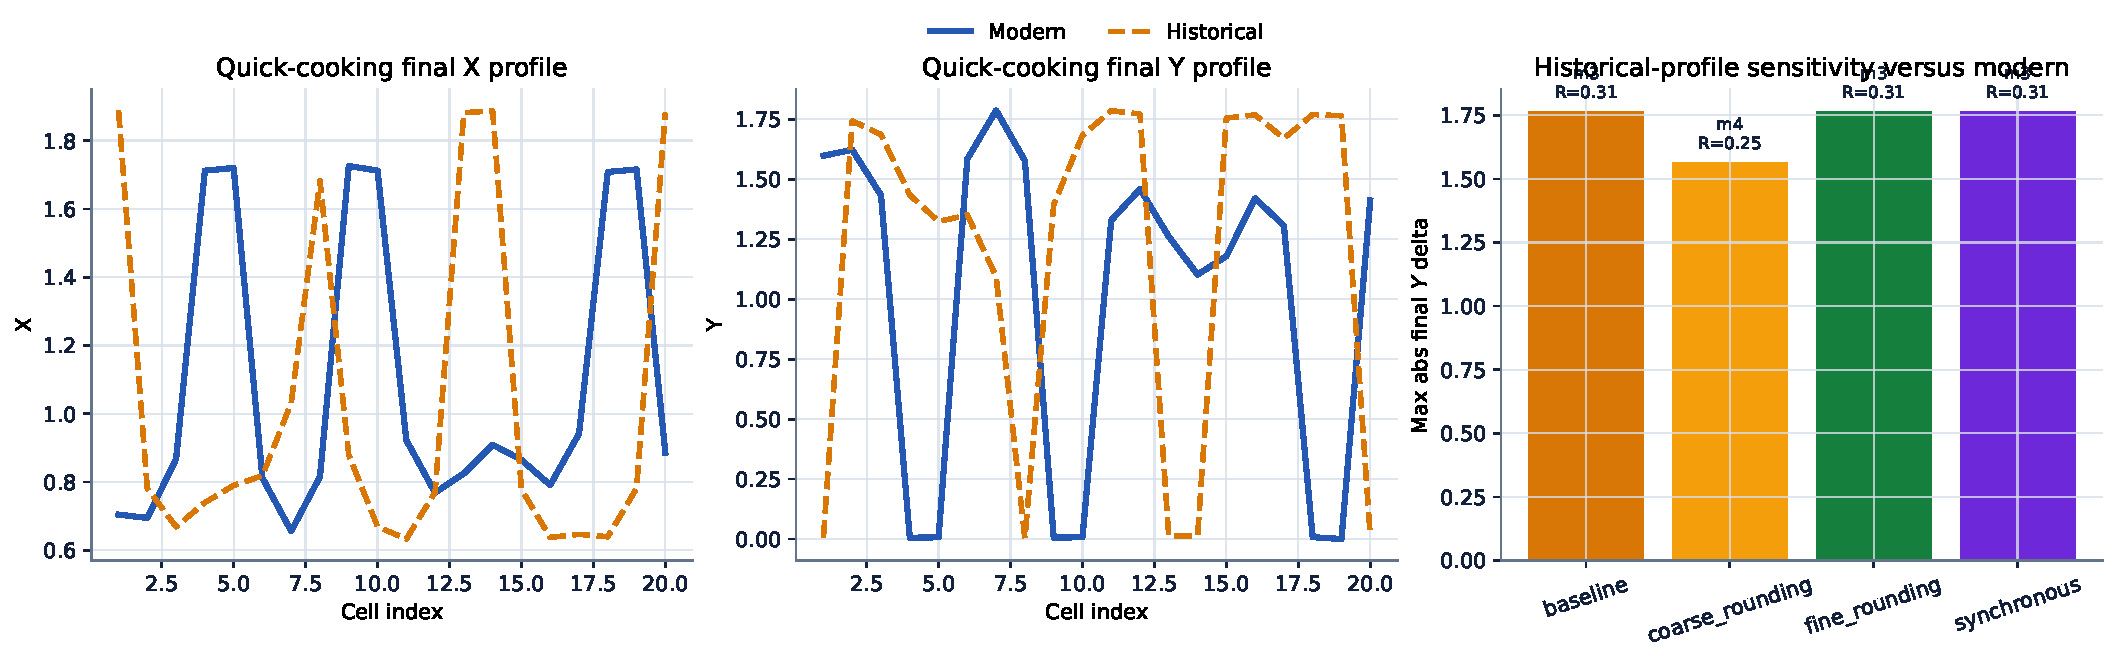
\includegraphics[width=0.94\linewidth]{figures/historical_quick_comparison.pdf}
    \caption{Modern versus paper-constrained historical quick-cooking final profiles.}
    \label{fig:historical}
\end{figure}

\noindent Figure~\ref{fig:historical} shows why the historical branch matters. The left two panels compare the modern quick-cooking final profiles against the baseline historical profile directly. The right panel shows that the choice of historical reconstruction assumptions matters internally as well: coarse rounding flips the quick-cooking winner from mode 3 to mode 4 and lowers regularity, while fine rounding and synchronous updating stay much closer to the baseline branch. This is exactly the right reading of the branch: it measures plausible historical sensitivity, not exact historical identity.

\section*{Hypothesis Verdict}
The Section 10 hypotheses remain the main explicit hypotheses in the repository.

\begin{description}
    \item[H1.] Supported. Homogeneity breaks under the prescribed reaction-diffusion dynamics.
    \item[H2.] Supported. Diffusion participates in the instability rather than merely smoothing it away.
    \item[H3.] Supported. The selected pattern is a low-order stationary finite-wave-length mode.
    \item[H4.] Supported. Microscopic stochastic disturbances are sufficient seeds for pattern divergence.
    \item[H5.] Supported. In quick cooking, mode 3 is the commonest outcome and mode 4 is the nearest rival.
    \item[H6.] Supported. Slow cooking strongly regularizes the pattern and nearly eliminates mode-4 wins.
\end{description}

\noindent\textbf{Overall verdict.} The repository now supports the original Section 10 hypothesis strongly and extends itself into a broader paper-example platform in a defensible way. Section 10 remains the best-validated historical reconstruction. The Table 2 and oscillatory branches are successful as explicit paper-facing workflows and toolkits, and the historical branch succeeds as sensitivity analysis, not exact emulation.

\section*{Limitations}
The main limitations are now clearer rather than smaller.
\begin{itemize}
    \item The Section 10 path is still the only part that has deep specimen-level validation against published numerical targets.
    \item The Table 2 stable-ring workflow still depends on an inferred forcing/stabilization term around the published six-cell profile. That is deliberate and documented, but it is not yet a full derivation from the reduced family law alone.
    \item The oscillatory presets are qualitative paper-matched toolkit examples rather than complete historical reconstructions.
    \item The historical branch is approximate and paper-constrained. The report, README, and SPEC all state that it is not an exact Manchester-machine emulator.
\end{itemize}

\section*{Artifacts}
The raw outputs used here are under \path{results/final_validation/}. Figure-generation outputs are under \path{results/hypothesis_figures/}. The full pipeline is scripted in \path{scripts/run_full_validation.sh}.

\end{document}
